\documentclass{article}
\usepackage[utf8]{inputenc}
\usepackage{float}
\usepackage[spanish]{babel}
\usepackage{graphicx}
\usepackage{listings}
\usepackage{color}
\usepackage{datetime}
\usepackage{csquotes}
\usepackage[table,xcdraw]{xcolor}
\documentclass[xcolor=table]{beamer}
\newdate{date}{02}{04}{2019}

\title{Tarea 4}
\author{Jesus Angel Patlán Castillo (5261)}
\date{\displaydate{date}}



\begin{document}

\definecolor{codegreen}{rgb}{0,0.6,0}
\definecolor{codegray}{rgb}{0.5,0.5,0.5}
\definecolor{codepurple}{rgb}{0.58,0,0.82}
\definecolor{backcolour}{rgb}{0.95,0.95,0.92}
 
\lstdefinestyle{mystyle}{
    backgroundcolor=\color{backcolour},   
    commentstyle=\color{codegreen},
    keywordstyle=\color{magenta},
    numberstyle=\tiny\color{codegray},
    stringstyle=\color{codepurple},
    basicstyle=\footnotesize,
    breakatwhitespace=false,         
    breaklines=true,                 
    captionpos=b,                    
    keepspaces=true,                 
    numbers=left,                    
    numbersep=5pt,                  
    showspaces=false,                
    showstringspaces=false,
    showtabs=false,                  
    tabsize=2
}
 
\lstset{style=mystyle}


\maketitle

En esta tarea se analizan la complejidad que se tiene en la utilización de métodos algoritmicos de flujo máximo en distintos tipos de grafos, los cuales son generados por algoritmos de generación de grafos proporcionados por libererias de Python. Los algoritmos se obtuvieron por medio de la librería NetworkX \cite{NetworkX} de Python \cite{Python}, la librería Matplotlib \cite{Matplotlib} es utilizada para generar las gráfica de correlación entre los efectos estudiados. El código empleado se obtuvo consultando la documentación oficial de la librería NetworkX \cite{NetworkXD}. Las imágenes y el código se encuentran disponibles directamente en mi repositorio \cite{JAPC}.

\section{Metodología}
La librería NetworkX tiene a la mano diversos algoritmos para resolver distintos algoritmos para poder resolver problemas de flujo máximo. Particularmente para esta investigación, se realiza el análisis de los algoritmos:
\begin{itemize}
\item{Flujo Máximo}: El algoritmo de flujo máximo nos permite encontrar el flujo máximo que se puede dar entre dos nodos del grafo (llamados fuente y sumidero). En la librería de NetworkX esta disponible por medio de  la función ``maximum flow(G,N1,N2)", donde el parámetro G es el grafo, N1 el nodo fuente y N2 el nodo sumidero:
\lstinputlisting[language=Python,firstline=68,lastline=68]{T4.py}
\item{Valor de flujo máximo}:  El algoritmo de valor de flujo máximo se utiliza para encontrar el valor máximo de flujo entre un par de nodos. En la librería de NetworkX esta disponible por medio de  la función ``maximum flow value(G,N1,N2)", donde el parámetro G es el grafo, N1 es el nodo fuente y N2 es el nodo sumidero:
\lstinputlisting[language=Python,firstline=73,lastline=73]{T4.py}
\item{Valor de corte mínimo}: El algoritmo valor de corte mínimo nos permite encontrar el valor mínimo entre el corte (una partición de vertices del grafo) que permita minimizar los pesos entre los grafos. En la librería de NetworkX esta disponible por medio de  la función ``minimum cut value(G,N1,N2)", donde el parámetro G es el grafo, N1 es el nodo fuente y N2 es el nodo sumidero:
\lstinputlisting[language=Python,firstline=78,lastline=78]{T4.py}
\end{itemize}
Cada uno de estos algoritmos fueron ejecutados sobre 10 grafos diferentes generados por 3 metodos de generación de grafos distinos, los cuales son:

\begin{itemize}
\item{Grafo paleta}: Un grafo paleta es un grafo que consiste en la unión entre un grafo completo y un ``puente" sobre uno de los nodos del grafo. En la librería de NetworkX esta disponible por medio de  la función ``lollipop graph(N1,N2)", donde el parámetro N1 es la dimensión del grafo completo y N2 es la dimensión del ``puente":
\lstinputlisting[language=Python,firstline=42,lastline=42]{T4.py}
\item{Grafo Turan}:  El grafo turan es un grafo completo multipartito de que contiene $n$ vertices con $r$ subconjuntos disjuntos. En la librería de NetworkX esta disponible por medio de  la función ``turan graph(n,r)", donde el parámetro n es la cantidad de vertices del grafo completo y r es la cantidad de subconjuntos disjuntos:
\lstinputlisting[language=Python,firstline=45,lastline=45]{T4.py}
\item{Grafo escalera}: El grafo escalera es un grafo que contiene dos caminos de $n$ nodos, sobre el cual cada par esta conectado por una única arista. En la librería de NetworkX esta disponible por medio de  la función ``ladder graph(n)", donde el parámetro n es la dimensión del grafo:
\lstinputlisting[language=Python,firstline=48,lastline=48]{T4.py}
\end{itemize}
Para cada combinación de métodos de flujo máximo y de generación de grafo, se realizaron 10 replicas de grafos distintos, para cada uno de los cuales se realizaron 5 repeticiones distintas para 5 pares de fuente-sumidero distintos. Además, se consideraron 4 distintos ordenes de tamaño para cada grafo, considerando una escala logarítmica en base $2^n$ con valores de $n \in {7,8,9,10}$. Después de realizar las replicas, se obtuvo el tiempo que tomo en ejecutar cada algoritmo en cada uno de los grafos, y se realizaron las pruebas estadísticas ANOVA para determinar si el tiempo de ejecución es afectado por el orden del grafo, el algoritmo de flujo máximo utilizado, el algoritmo generador del grafo y la densidad de cada grafo; y si existe una correlación entre estos factores.
Las siguientes líneas de código representan la generación de la recopilación de datos de las replicas, la matriz de correlación y la tabla de ANOVA:
\lstinputlisting[language=Python,firstline=36]{T4.py}

Este proceso se realizó en una laptop con las siguientes características:
\begin{itemize}
\item{Procesador}: Intel Core i7-7500U 2.7GHz
\item{Memoria RAM}: 16GB 
\item{Sistema Operativo}: Windows 10 64 bits
\end{itemize}
\section{Resultados}
Se obtuvieron los siguientes resultados de las replicas, una matríz de correlación en la figura \ref{fig:matriz} y las pruebas estadísticas de ANOVA para determinar los efectos de los factores:

\begin{figure}[H]
    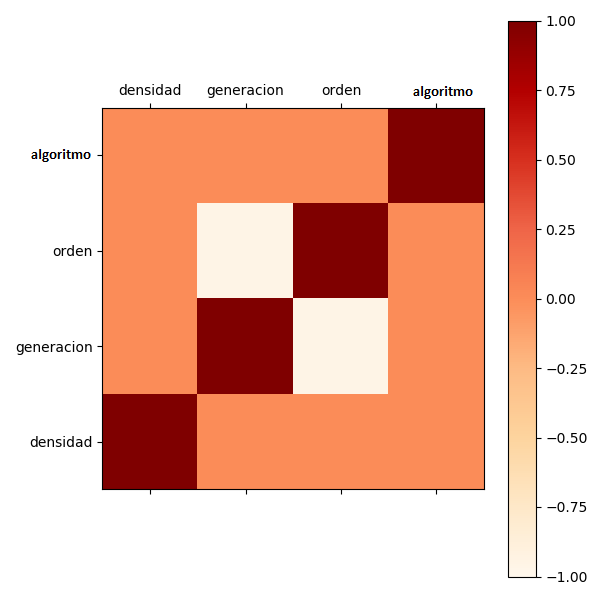
\includegraphics[width=\textwidth]{matriz}
    \caption{Matriz de correlación.}
    \label{fig:matriz}
\end{figure}
\begin{table}[H]
\begin{tabular}{|
>{\columncolor[HTML]{ECF4FF}}r |c|c|}
\hline
\textbf{ANOVA}                               & \cellcolor[HTML]{ECF4FF}\textbf{Grados de Libertad} & \cellcolor[HTML]{ECF4FF}\textbf{Valor P} \\ \hline
\textbf{C(generation)}                                   & 2                                  & 6.06E-102                         \\ \hline
\textbf{C(algoritmo)}                                    & 2                                  & 0.155326227                       \\ \hline
\textbf{C(orden)}                                        & 3                                  & 1.41E-221                         \\ \hline
\textbf{C(densidad)}                                     & 11                                 & 0                                 \\ \hline
\textbf{C(generation):C(algoritmo)}                      & 4                                  & 0.49355476                        \\ \hline
\textbf{C(generation):C(orden)}                          & 6                                  & 0                                 \\ \hline
\textbf{C(algoritmo):C(orden)}                           & 6                                  & 0.338715638                       \\ \hline
\textbf{C(generation):C(densidad)}                       & 22                                 & 0.99244162                        \\ \hline
\textbf{C(algoritmo):C(densidad)}                        & 22                                 & 2.37E-77                          \\ \hline
\textbf{C(orden):C(densidad)}                            & 33                                 & 0.999058669                       \\ \hline
\textbf{C(generation):C(algoritmo):C(orden)}             & 12                                 & 7.24E-27                          \\ \hline
\textbf{C(generation):C(algoritmo):C(densidad)}          & 44                                 & 0.997362183                       \\ \hline
\textbf{C(generation):C(orden):C(densidad)}              & 66                                 & 7.24E-27                          \\ \hline
\textbf{C(algoritmo):C(orden):C(densidad)}               & 66                                 & 0.973080866                       \\ \hline
\textbf{C(generation):C(algoritmo):C(orden):C(densidad)} & 132                                & 0.999714748                       \\ \hline
\textbf{Residual}                                        & 1764                               &                                   \\ \hline
\end{tabular}
\end{table}
\section{Conclusiones}
Como conclusión de esta investigación, se tiene que cada uno de los factores de algoritmo, orden, generación de grafo y densidad afectan directamente con el tiempo de ejecución de los algoritmos, además que, en combinación, todos excepto la combinación de orden-generación afectan al rendimiento del algoritmo. La tabla ANOVA respalda los resultados con los valores de P dados.
\bibliographystyle{plain}
\bibliography{references}

\end{document}
